\section{Introducción}


\subsection{Comparación de Rendimiento entre Goland, Python y C++}
En este trabajo, se llevará a cabo una comparación entre tres lenguajes de programación ampliamente utilizados: Go (Goland), Python y C++. El objetivo de esta comparación es evaluar el tiempo de procesamiento de cuatro programas implementados en cada uno de estos lenguajes.

El tiempo de procesamiento es un factor crucial en el rendimiento de un programa, ya que determina cuánto tiempo lleva ejecutar un conjunto de instrucciones y completar una tarea específica. La eficiencia en el tiempo de procesamiento es especialmente relevante en aplicaciones que manejan grandes cantidades de datos o realizan cálculos intensivos.

Para realizar la comparación, implementaremos cuatro programas con funcionalidades similares en cada uno de los lenguajes mencionados. Estos programas serán diseñados para realizar tareas representativas y representativas de cada lenguaje.

En cada caso, mediremos el tiempo de procesamiento de los programas utilizando herramientas adecuadas para obtener resultados precisos y comparables. La medición se realizará ejecutando cada programa varias veces y tomando el promedio para obtener un tiempo representativo.

Al comparar los resultados obtenidos, podremos evaluar cómo cada lenguaje maneja las tareas específicas y determinar cuál es más eficiente en términos de tiempo de procesamiento. Además, esta comparación nos permitirá identificar las fortalezas y debilidades de cada lenguaje para diferentes tipos de aplicaciones y escenarios de uso.

Es importante destacar que la eficiencia en el tiempo de procesamiento es solo uno de los muchos factores que deben tenerse en cuenta al elegir un lenguaje de programación. Otros aspectos como la facilidad de uso, la legibilidad del código, el ecosistema de bibliotecas y la comunidad de desarrollo también son consideraciones importantes.

En resumen, este estudio comparativo proporcionará información valiosa sobre el rendimiento en tiempo de procesamiento de Go, Python y C++, lo que permitirá a los desarrolladores tomar decisiones informadas al elegir el lenguaje más adecuado para sus proyectos y requisitos específicos.
\section{Algoritmos}
.Bubble Sort:
Bubble Sort es un algoritmo simple de ordenación que funciona comparando repetidamente elementos adyacentes y haciendo intercambios si están en el orden incorrecto. El proceso se repite hasta que no se realicen más intercambios, lo que indica que la lista está completamente ordenada. Aunque es fácil de implementar, Bubble Sort no es eficiente para listas grandes

\begin{figure}[h]
    \centering
    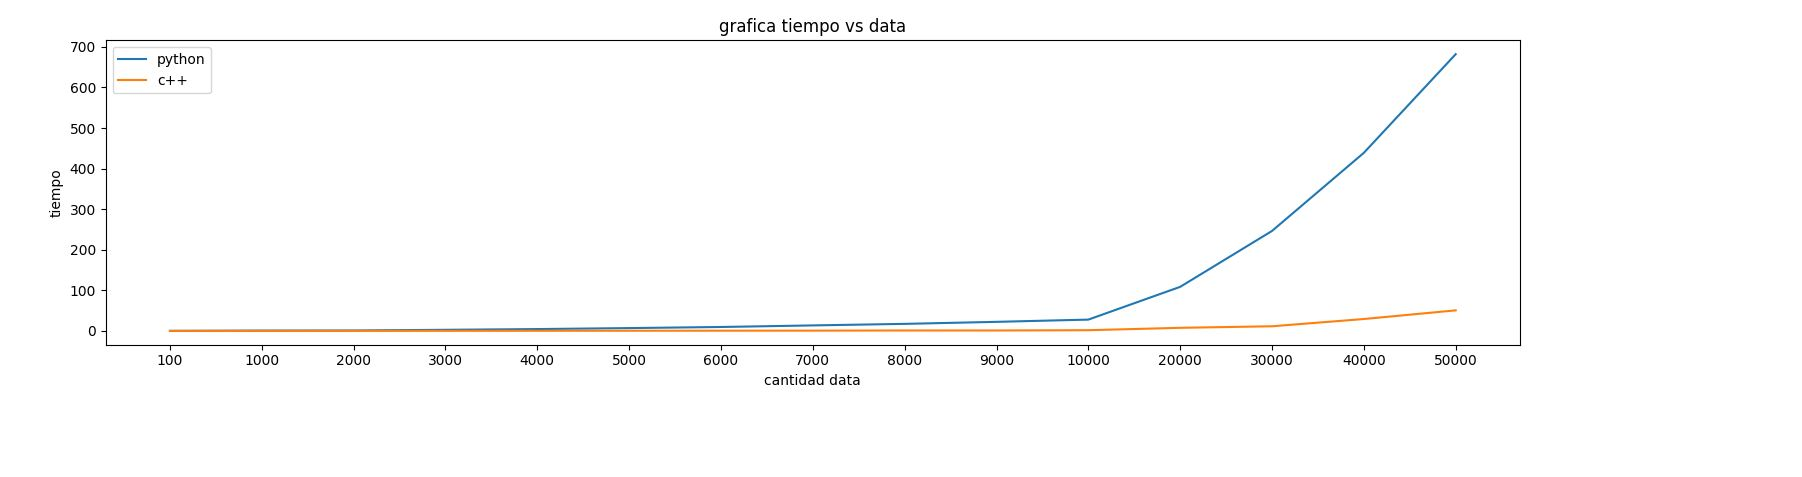
\includegraphics[scale=0.4]{images/1.JPG}
    \label{fig:imagen}
\end{figure}

Merge Sort:
Merge Sort es un algoritmo de ordenación basado en la técnica "divide y vencerás". Divide la lista no ordenada en sublistas más pequeñas, las ordena de forma recursiva y luego las combina para obtener la lista ordenada final. Merge Sort tiene una complejidad promedio de O(n log n), lo que lo hace mucho más eficiente que Bubble Sort para grandes conjuntos de datos. Es ampliamente utilizado en aplicaciones que requieren una ordenación estable y eficiente.
\begin{figure}[h]
    \centering
    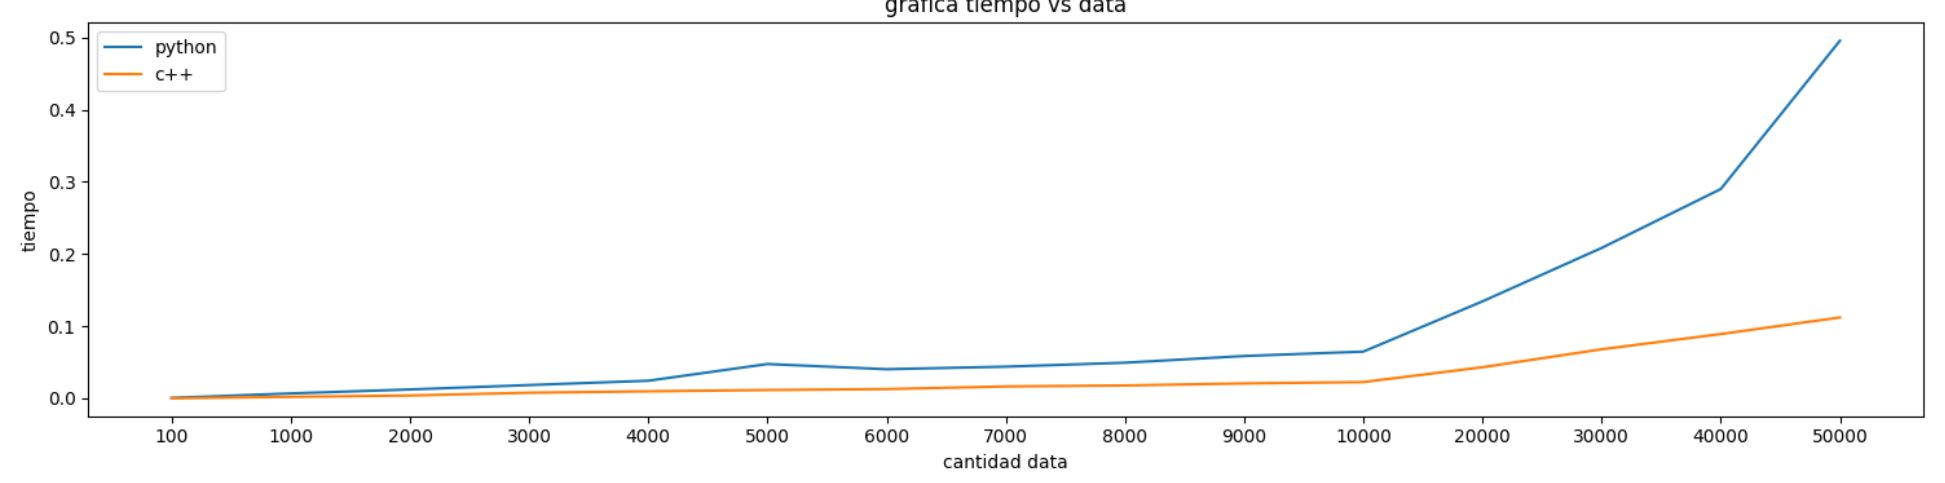
\includegraphics[scale=0.3]{images/2.JPG}
    \label{fig:imagen}
\end{figure}

Quick Sort:
Quick Sort es otro algoritmo de ordenación "divide y vencerás" que utiliza una estrategia de partición para ordenar los elementos. Selecciona un elemento como "pivote" y divide la lista en dos subconjuntos: uno con elementos menores que el pivote y otro con elementos mayores. Luego, aplica recursivamente el mismo proceso a los dos subconjuntos. Quick Sort tiene una complejidad promedio de O(n log n) y, en general, es más rápido que Merge Sort para conjuntos de datos más pequeños.

\begin{figure}[h]
    \centering
    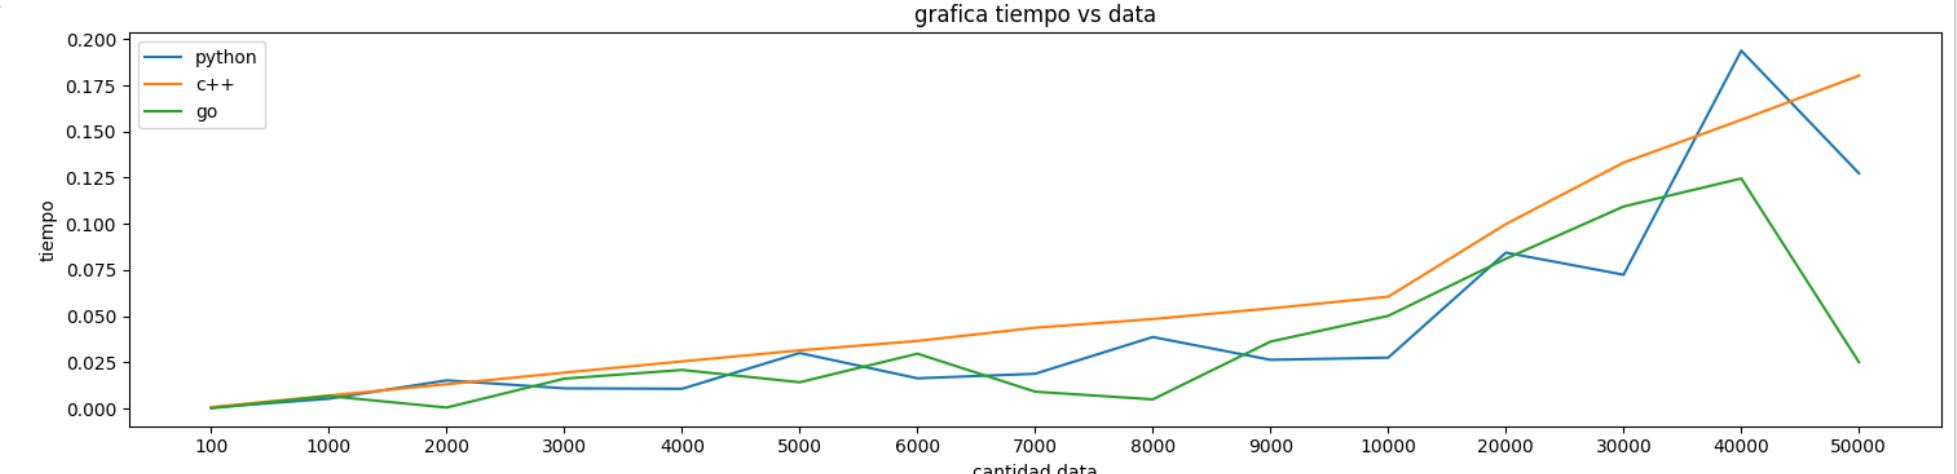
\includegraphics[scale=0.3]{images/3.JPG}
    \label{fig:imagen}
\end{figure}

Selection Sort:
Selection Sort es un algoritmo de ordenación que busca el elemento más pequeño en cada iteración y lo coloca en su posición correcta. Comienza seleccionando el elemento más pequeño y lo intercambia con el primer elemento. Luego, busca el siguiente elemento más pequeño y lo coloca en la segunda posición, y así sucesivamente.En resumen, cada algoritmo de ordenación tiene sus ventajas y desventajas en términos de eficiencia y facilidad de implementación. La elección del algoritmo de ordenación adecuado dependerá del tamaño del conjunto de datos y los requisitos de rendimiento del problema específico que estés abordando.

\begin{figure}[h]
    \centering
    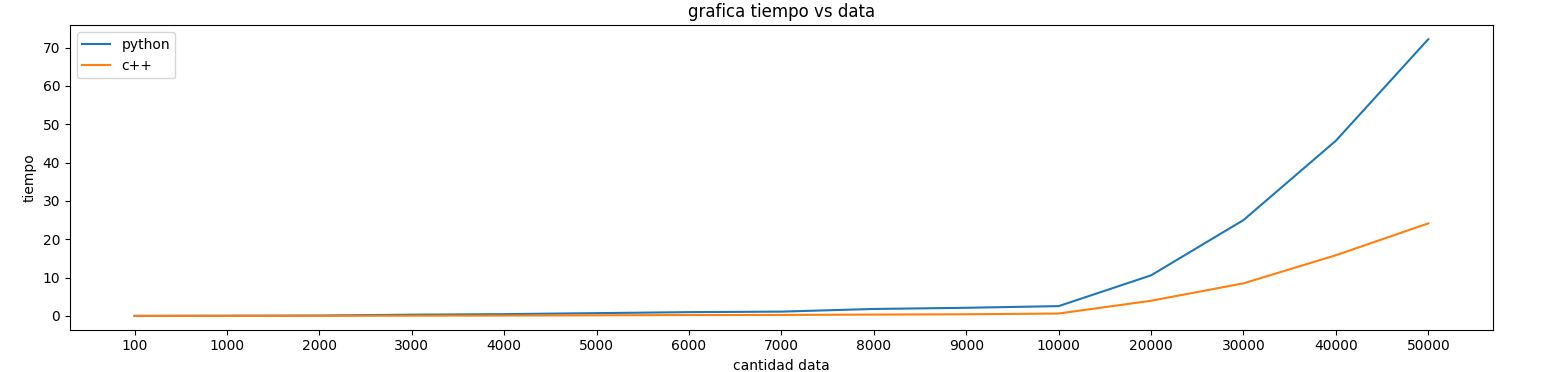
\includegraphics[scale=0.4]{images/4.JPG}
    \label{fig:imagen}
\end{figure}

\section{Implementación}

\href{https://github.com/jhoel-choque/practica_1.git}{Enlace git hub:}

\section{Resultados}
Al realizar la comparación entre los lenguajes de programación Go (Goland), Python y C++ en términos de tiempo de procesamiento, se pueden obtener varias conclusiones dependiendo de las características de los programas y los conjuntos de datos utilizados en los experimentos. Aquí hay algunas posibles conclusiones:

1. Rendimiento y Eficiencia: C++ suele tener un rendimiento y eficiencia superiores en comparación con Python y Go. Esto se debe a que C++ es un lenguaje compilado y altamente optimizado, mientras que Python y Go son lenguajes interpretados y tienen una mayor sobrecarga de tiempo de ejecución.

2. Facilidad de Uso y Desarrollo: Python y Go son lenguajes más fáciles de aprender y utilizar que C++. Python se destaca por su simplicidad y legibilidad, lo que facilita el desarrollo rápido de prototipos y la implementación de algoritmos. Go, por su parte, proporciona una sintaxis limpia y fácil de entender, además de ser fuertemente tipado.

3. Paralelismo y Concurrencia: Go está diseñado con el paralelismo y la concurrencia en mente, lo que le da ventaja en términos de rendimiento en tareas concurrentes y distribuidas. Python también ofrece opciones de concurrencia, pero Go está más enfocado en este aspecto.

4. Uso de Recursos: En general, Python puede consumir más recursos en comparación con Go y C++. Esto se debe a la naturaleza interpretada de Python y a su mayor sobrecarga en tiempo de ejecución. Go, por otro lado, es conocido por su baja sobrecarga de tiempo de ejecución y su gestión eficiente de recursos.

5. Bibliotecas y Ecosistema: Python tiene una amplia variedad de bibliotecas y módulos disponibles para diversas tareas, lo que facilita el desarrollo de aplicaciones y el acceso a funcionalidades adicionales. Go también tiene un ecosistema en crecimiento, pero puede tener menos bibliotecas disponibles en comparación con Python. C++, por su parte, tiene una gran cantidad de bibliotecas y es ampliamente utilizado en aplicaciones de alto rendimiento.

En general, la elección del lenguaje de programación dependerá de los requisitos específicos del proyecto, el tamaño del conjunto de datos y la naturaleza del problema que se va a resolver. Cada lenguaje tiene sus ventajas y desventajas, y es importante seleccionar el lenguaje más adecuado para cada caso particular. La medición del tiempo de procesamiento de los programas implementados en los tres lenguajes proporcionará datos cuantitativos para respaldar la elección del lenguaje más adecuado para el problema en cuestión.

\subsection{Subsection1}


\section{Conclusiones}